\section{Hilbert spaces}
\subsubsection{(def) }
$H$ (real) vector space. A function
$$p:H\times H\xrightarrow[\quad]{} \mathbb R$$
is a scalar product (or inner product) if it satisfies the following properties:
\begin{itemize}
    \item positivity: $p(x,x)>0\quad \forall x, \quad p(x,x)=0\iff x=0$
    \item simmetry: $p(x,y)=p(y,x)\quad \forall x,y$
    \item bilinearity: $p(\alpha_1x_1+\alpha_2x_2,y)=\alpha_1 p(x_1,y)+\alpha_2p(x_2,y)$
\end{itemize}
\paragraph{Notation} $p(x,y)=\scalar xy=(x,y)=x\cdot y$
\subsubsection{(def)}
$(H,\scalar \ \ )$ is a pre-Hilbertian pace (an inner product space).
\subsubsection{(prop)}
$(H,\scalar \ \ )$ inner product space. Then:
\begin{enumerate}
    \item $|\scalar xy|\leq \sqrt{\scalar xx}\cdot \sqrt{ \scalar yy}$ (Cauchy-Schwartz inequality)
    \item define $\Vert x\Vert =\sqrt{\scalar xx}$, the induced norm.
    It is a norm on $H$ and $(H,\cnorm)$ is a normed space.
    \item Parallelogram identity
    $$\Vert x+y\Vert ^2 +\Vert x-y\Vert ^2=2\Vert x\Vert ^2 +2 \Vert y\Vert ^2$$
\end{enumerate}
\begin{proof}\ 
    \begin{enumerate}
        \item Same as in $\mathbb R^n$
        \item exercise (triangular inequality $\impliedby$ Cauchy-Schwartz)
        \item $\scalar{x\pm y}{x \pm y}=\Vert x\Vert ^2\pm 2\scalar xy +\Vert y\Vert ^2$
    \end{enumerate}
\end{proof}
\paragraph{Remark}
\begin{itemize}
    \item $(H,\scalar\ \ )$ inner product space
    \item $H,\cnorm )$ normed vector space
    \item $(H, d)$ metric space
\end{itemize}
\subsubsection{(def)}
$(H,\scalar\ \ )$, inner product space, is a Hilbert space if it is complete with respect to the induced norm (i.e. $(H,\cnorm)$ is Banach).
\paragraph{Examples}
\begin{enumerate}
    \item $\mathbb R^n$, euclidean scalar product 
    \item $L^2(X,\mathcal M,\mu)$,
    $$\scalar uv _{L^2}=\int_Xuv\ \mathrm d\mu$$
    $$\Vert u\Vert_2=\sqrt{\scalar uu}=\Big ( \int_Xu^2\ \mathrm d\mu\Big )^{\frac 12}$$
    ( $v,u\in l^2\implies \scalar vu_{l^2}=\sum_{k\in \mathbb N}u^{(k)}v^{(k)}$)
\end{enumerate}
\paragraph{Remark}
$\Big (C([a,b]), \scalar \ \ _{L^2}\Big )$ is a inner product space but not Hilbert.

\paragraph{Remark}
We know that $H$ Hilbert $\implies H$ Banach.
What can we say about the converse?
That is, is it possible to detect if in $(X,\cnorm)$, $\cnorm$ is induced by some product space?
\subsubsection{(prop)}
$(X,\cnorm)$ Banach. Then it is also Hilert $\iff$ $\cnorm$ satisfies the parallelogram, with $\scalar xy = \frac 14 (\Vert x+y\Vert ^2-\Vert x-y\Vert ^2)$
\paragraph{Exercise} Cons: we can check that:
\begin{itemize}
    \item $(L^p,\cnorm_p)$ is not Hilbert for $p\neq 2$
    \item $(C,\cnorm)$ is not Hilbert 

\end{itemize}
\subsubsection{(def)}
\begin{itemize}
    \item Two vectors $x,y\in H$ are orthogonal $\iff \scalar xy=0$ (notation: $y\perp x$)
    \item given $V\subset H$, the orthogonal complement is $$V^{\perp}=\{w\in H:\scalar wv =0 \quad \forall v\in V^{\perp}\}$$
\end{itemize}
\subsection{Orthogonal projections}
\paragraph{Recall}
\begin{itemize}
    \item $S\subset H$ is convex if $x,y\in S\implies tx+(1-t)y\in S$, $0\leq t\leq 1$
    \item $S\subset H, \ x\in H$
    $$\mathrm{dist}(x,S)=\inf_{v\in S}\Vert x-v\Vert$$
\end{itemize}
\subsubsection{(thm) Projection Theorem on Closed Convex Sets}
Consider:
\begin{itemize}
    \item $H$ Hilbert
    \item $x\in H$
    \item $S\subset H$ closed, convex (non-empty)
\end{itemize}
$\exists ! h\in S$ such that:
\begin{enumerate}
    \item $$\Vert x-h\Vert =\mathrm{dist}(x,S)=\inf_{v\in S}\Vert x-v\Vert $$
    Moreover, $h$ is carachterized by the "variational inequality"
    \item $\scalar{x-h}{v-h}\leq 0\quad \forall v\in S$
\end{enumerate}
$h\in S$ satisfies (1) $\iff $ satisfies (2)
\begin{proof}
    $0\leq d=\inf_{v\in S} \Vert x-v\Vert$\\
    Take a "minimizing sequence"\\
    $d\leq \Vert x-v_n\Vert \leq d+\frac 12\quad \forall n$
    \\
    We are going to show that $\{v_n\}_n$ is Cauchy applying the parallelogram identity to $x-v_n$, $x-v_m$.
    $$\Vert x-v_n+x-v_m\Vert ^2+\Vert x-v_n-x+v_m\Vert ^2=2\Vert x-v_n\Vert ^2+2\Vert x-v_m\Vert ^2$$
    (i.e. $0\leq\Vert v_n-v_m\Vert ^2 \leq 2\Vert x-v_n\Vert ^2+2\Vert x-v_m\Vert ^2-4d^2\to 0$
    $\implies \{v_n\}_n$ is a Cauchy sequence\\
    $$H \text{ Hilbert} \implies \exists h\in H\text{ s.t. } v_n\to h \text { in }H \text{ as }n \to +\infty$$
    $$S \text{ closed}: \begin{cases}
        \{v_n\}_n\subset S\\ v_n\to h \in H
    \end{cases}\implies h\in S$$
    Finally, $d\leq \Vert x-v_n\Vert \leq d+\frac 1n$, for $n\to+\infty$, $d\leq \Vert x-v_n\Vert \leq d=\mathrm{dist}(x,S)$
\end{proof}
\paragraph{Remark}
To prove uniqueness, use the parallelogram identity, with $x-h_1$ and $x-h_2\implies h_1=h_2$
\paragraph{Relevant case} Any $V\subset H$ subspace is convex.
\paragraph{Projection theorem on closed subspaces}
Consider $H$ an Hibert space, $x\in H$ and $V\subset H$ closed subspace.\\
Then $\exists ! \ h\in V:\Vert x-h\Vert =\inf_{v\in V} \Vert x-v\Vert $ (1)\\
Moreover, $h\in V$ satisfies the above condition $\iff$ it satisfies:
$$\scalar{x-h}v=0\quad \forall v\in V$$
\paragraph{Remark} $x-h\perp v \quad \forall v\in V$ (i.e. $x-h\in V^\perp$
\begin{figure}[H]
    \centering
    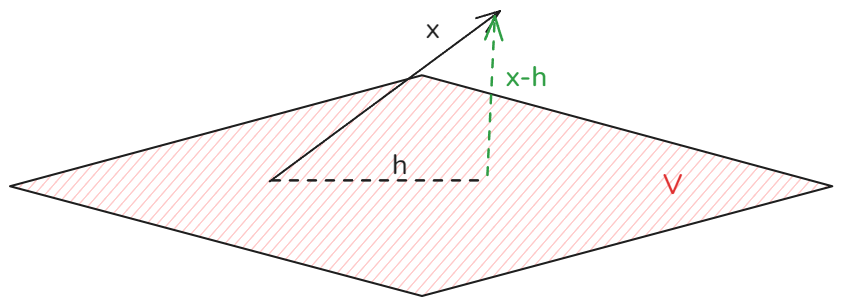
\includegraphics[width=0.5\linewidth]{image.png}
    \caption{Enter Caption}
    \label{fig:enter-label}
\end{figure}
\paragraph{Remark (on closed subspaces)}
Consider $H$ an Hilber space and a subspace $V\subset H$.
For sure $V$ is \textbf{closed} if 
\begin{itemize}
    \item its dimension is finite. $V<+\infty$
    \item $V=Ker(L)$, with $L\in \mathcal L(H,Y)$
    \item $V^\perp$ is always a closed subspace, whichever $V$ is. (continuity of the scalar product).
\end{itemize}
The consequence of this, if we take the orthogonal of the orthogonal, we get the closure of the initial space.
$$\Big ((V)^\perp\Big)^\perp =\overline V$$
$V$ is never closed if:
\begin{itemize}
    \item $V\subsetneq H$ dense. (for a dense subspace, the orthogonal is always $\{0\}\implies (V^\perp)^\perp =H=\overline V$)
\end{itemize}
\subsubsection{(thm)}
Consider $H$ Hilbert, $V\subset H$ closed subspace, then:
\begin{enumerate}
    \item $\forall x \in H, \quad x=P_Vx+P_{V^\perp}x$
    \item $x\in V\iff x=P_Vx$
    \item $|x|^2=\Vert P_Vx\Vert ^2+\Vert P_{V^\perp} x\Vert ^2$
    \item $P_V, \ P_{V^\perp}\in \mathcal L(H)$ and their norm is 1.
\end{enumerate}
\subsection{Dual of a Hilbert Space}
Consider $H$ Hilber space, take any vector $u\in H$, define $L_u\in H^*$, $L_uv\coloneqq \scalar uv,\quad \forall v\in H$\\
Then $L_u$ is linear.
$$\Vert L_u\Vert _*=\sup_{x\neq 0}\frac{|L_ux|}{\Vert x\Vert }=\sup_{x\neq 0}\frac{|\scalar ux|}{\Vert x\Vert} $$
\begin{itemize}
    \item $$\sup_{x\neq 0}\frac{|\scalar ux|}{\Vert x\Vert}\leq \sup_{x\neq 0}\frac{\Vert u\Vert \Vert x\Vert}{\Vert x\Vert}=\Vert u\Vert$$
    \item $$\sup_{x\neq 0}\frac{|\scalar ux|}{\Vert x\Vert}\geq \frac{\scalar uu}{\Vert u\Vert}=\Vert u\Vert$$
\end{itemize}
$$\implies \Big \Vert L_u\Big \Vert _*=\Vert u\Vert $$
(that means that it is isometric).\\
We obtain $i:H\xrightarrow[\quad]{} H^*$, $u \xrightarrow[\quad]{}L_u$
\subsubsection{(thm) Riesz's Representation Theorem (in Hilbert spaces)}
$H$ Hilbert, $\forall L\in H^*, \exists !u\in H, \ s.t.$
$$Lv=\scalar uv \quad \forall v\in H$$
Moreover, $\Vert u\Vert =\Vert L\Vert_*$ (i is an isometric isomorphism).
\paragraph{Corollary} $H$ Hilbert $\implies H$ Reflexive
$$H\simeq H^*\implies H^*\simeq H^{**}$$
\paragraph{Remark}
We can identify $H$ and $H^*$, but depending on $\scalar\cdot\cdot$. So $V\subsetneq H$ subspace, dense Hilbert,
$$V^*\supsetneq H^*$$
\paragraph{Remark}
The Riesz Representation Theorem is a "well-posed" theorem.
Consider the problem:
\begin{itemize}
    \item Given $L\in H^*$, find $u\in H$ s.t. $\scalar uv =Lv\quad \forall v\in H$
\end{itemize}
Riesz $\implies \exists !\ u$, and $\Vert u\Vert =\Vert L\Vert _*\implies \Vert u_1-u_2\Vert =\Vert L_1-L_2\Vert _*$
\begin{proof}\ 
Let's prove existance: we distinguish two cases:
\begin{enumerate}
    \item Assume $Ker (L)=H$. Just take $u=0$
    $$\scalar 0,v =0=Lv$$
    \item $\exists z_0\in H\setminus Ker(L) \implies Lz_0\neq 0$ and $z_0\neq 0$\\
    Since $Ker(L)$ is a closed subspace of $H$,
    $$z\coloneqq \frac{P_{(Ker(L))^\perp}z_0}{\Vert {P_{(Ker(L))^\perp}z_0\Vert}}\implies \begin{cases}
        \Vert z\Vert =1\\ z\in (Ker(L))^\perp
    \end{cases}$$
    Take $v\in H$ and $w =v-\frac{Lv}{Lz}z$ so that $Lw=0$\\
    Since
    \begin{itemize}
        \item $w \in Ker(L)$
        \item $z\in (Ker(L))^\perp$
    \end{itemize}
    $$\implies 0=\scalar wz = \scalar{v-\frac{Lv}{Lz}z}{z}=\scalar vz \frac{Lv}{Lz}\scalar zz = \scalar zv -\frac{Lv}{Lz}$$
    i.e. $$Lv=Lz\scalar zv =\scalar{(Lz)z}v \quad \forall v\in H$$
\end{enumerate}
Let $u_1,\ u_2\in H$ s.t. 
$$Lv=\scalar{u_1}v \quad \forall v\in H$$
$$Lv=\scalar{u_2}v \quad \forall v\in H$$
$$\scalar{u_1-u_2}v=0 \quad \forall v\in H$$
Take $v=u_1-u_2$
$$\Vert u_1-u_2\Vert^2=0\implies u_1=u_2$$
Finally, $\Vert u\Vert = \Vert L\Vert _*$ by the discussion above (both equal to $\Vert L_u\Vert_*$
\end{proof}
\paragraph{Consequences}
Consider $H$ Hilbert space, and $\{ x_n\}_n\subset H$. Then $x_n \rightharpoonup x$ weakly in $H$.
$$\iff \scalar u{x_n}\to \scalar ux \quad \forall u\in H$$
Moreover, by reflexivity, $\{x_n\}_n\subset H$ bounded.
$$\implies x_{n_k}\rightharpoondown x\quad \text{(Banach Alaogh 1)}$$
Sometimes, weak convergence + more conditions $\implies$ strong convergence. For instance,
\subsubsection{(prop)}
Consider $H$ Hilbert space, $\{x_n\}_n\subset H$. Assume 
$$\begin{cases}
    x_n\rightharpoonup x\text{ weakly in } H\\
    \Vert x_n\Vert \to \Vert x\Vert
\end{cases}$$
Then $x_n\to x$ strongly in $H$.
\begin{proof}
    $0\leq \Vert x_n-x\Vert ^2=\Vert x_n\Vert^2-2\scalar {x_n}x +\Vert x\Vert ^2$
    We have that:
    \begin{itemize}
        \item $\Vert x_n\Vert^2\to \Vert x\Vert$
        \item $2\scalar {x_n}x \to 2\Vert x\Vert^2$
    \end{itemize}
    $\implies \xrightarrow[n\to+\infty]{}0$
\end{proof}
\subsection{Orthonormal basis}
Consider $H$ Hilbert.\\
\paragraph{Definition}
A sequence $\{ e_n\}_{n\in \mathbb N}\subset H$ is called an orthonormal basis for $H$ if:
\begin{itemize}
    \item $\Vert e_n\Vert =1, \ \scalar{e_i}{e_j}=0\quad \forall i\neq j$
    \item $\mathrm{span}(\{e_n\}_{n\in \mathbb N})$ is dense in $H$ (i.e. $H=\overline{\mathrm{span}(\{e_n\}_{n\in \mathbb N})}$
\end{itemize}
\paragraph{Examples}

\begin{enumerate}
    \item $H=l^2$
\begin{itemize}
    \item $e_1=(1,0,0,0,0,\dots)$
        \item $e_2=(0,1,0,0,0,\dots)$
    \item $e_3=(0,0,1,0,0,\dots)$

\end{itemize}
\item $H=L^2(-\pi,\pi)$
We can consider the Fourier series coefficients...
$$\Big\{\frac 1{\sqrt {2x}},\frac{\sin nx}{\sqrt{\pi}},\frac{\cos nx}{\sqrt{\pi}},\dots\Big\}$$
\end{enumerate}
\subsubsection{(thm)}
Every separable Hilbert space $H$ has an orthogonal basis.
\subsubsection{(thm)}
Let $\{e_n\}_n\subset H$ be an orthonormal basis, then:
\begin{enumerate}
    \item $\forall u\in H$, $$
    u=\sum_{n=1}^{+\infty} \scalar{u}{e_n} e_n$$
    ($\scalar{u}{e_n} $ Generalized Fourier Coefficients),\\
    and $$\Vert u\Vert ^2=\sum_{k=1}^{+\infty} |\scalar{u}{e_k}|^2 \quad \text{(Parseval-Bessel identity)}$$ 
\item Conversely: $\{ \alpha_n\}_{n\in \mathbb N}\in l^2$, then $\sum_{n=1}^{+\infty}\alpha_ne_n=x\in H$, with $\scalar x{e_n}=\alpha_n$
\end{enumerate}
\subsubsection{(prop)}
Consider any $\{e_n\}_n\subset H$ orthonormal basis,\\
Then
$$e_n\rightharpoonup 0 \text{ weakly in } H$$ but  $$e_n\centernot \to 0 \text{ strongly}$$
\begin{proof}
    By the Theorem, $\forall u \in H$, the series
    $$\sum_n |\scalar u{e_n}|^2<+\infty\implies \scalar u{e_n}\xrightarrow[n\to +\infty]{}0\quad \forall u\in H$$
    $\implies$ weak convergence ($e_n\rightharpoonup0$).\\
    But $\Vert e_n\Vert=1\centernot\to \Vert 0\Vert$
\end{proof}
\section{Spectral Theory}
Consider $E$ Banach and $T\in \mathcal L(E)=\mathcal (E,E)$
$$Tx=\lambda x$$
\subsection{(def)}
\begin{itemize}
    \item The resolvent set of $T$ is 
    $$\rho(T)=\{\lambda\in \mathbb R:T-\lambda I\text{ is bijective}\}$$
    \item The spectrum of $T$ is
    $$\sigma(T)=\mathbb R\setminus \rho(T)=\{\lambda \in \mathbb R: T-\lambda I\text{ is not bijective}\}$$
    \item $\lambda$ is an eigenvalue if
    $$Ker(T-\lambda I)\neq \{0\}$$
    and 
    $$EV(T)=\{\text{eigenvalues of }T\}\subset \mathbb R$$
\end{itemize}
\paragraph{Remark}
$$EV(T)\subset \sigma(T)$$
If $\dim(E)<+\infty$, then $EV(T)=\sigma(T)$\\
If $\dim(E)=+\infty$, then the strict inclusion may happen.
\subsubsection{(thm)}
Take a Banach space $E$ and a linear and continuous operator $T\in \mathcal L(E)$. Then:
\begin{enumerate}
    \item $\sigma_i(T)\subset \Big[-\Vert T\Vert_{\mathcal L(E)},\Vert T\Vert_{\mathcal L(E)}\Big]$
    \item $\sigma(T)$ is closed
\end{enumerate}
\paragraph{Remark}
The first point means that the "spectral radius" is always $\leq$ thant the operator norm of $T$
\paragraph{Remark}
If $|\lambda |>\Vert T\Vert_{\mathcal L(E)}\implies T-\lambda I$ is invertible. Moreover, $\rho(T)$ is open.
\paragraph{Example}
$E=l^2$\\
The "left shift operator" $T_l:l^2\to l^2$
$$\Big (T_l\ x\Big)^{(k)}=x^{k+1}$$
$x=(x^{(0)},x^{(1)},x^{(2)},\dots)$
$$T_l\ x=(x^{(1)},x^{(2)},x^{(3)},\dots)$$
Then 
\begin{itemize}
    \item one can prove that $T_l\in \mathcal L(l^2)$ and $\Vert T_l\Vert_{\mathcal L(l^2)}=1$\\
By the theorem, $\sigma (T_l)\subset [-1,1]$, closed.
\item continua
\end{itemize}

$R(T_l)=l^2$\\
$Ker(T_l)=\{ x: x^{(k)}=0\quad \forall k\geq1,\quad x^{(0)}\in \mathbb R\}$
and $\lambda=0$ is an eigenvalue of multiplicity 1.
\begin{itemize}
    \item Let's look for eigenvalues:\\
    $\lambda \in \mathbb R$ is an eigenvalue $\iff \exists x\neq 0$ s.t.
    $$L_l\ x=\lambda x$$
    $$\iff \Big(T_l\ x\Big)^{(k)}=\lambda x^{(k)}\quad \forall k\geq 0$$
    $$\iff x^{(k+1)}=\lambda x^{(k)}\quad \forall k\geq 0$$
    Take any $x^{(0)}=x_0\neq0$,\\
    $x^{(1)}=\lambda x_0$\\
    $x^{(2)}=\lambda x^{(1)}=\lambda ^2x_0$\\
    $\vdots$\\
    $x^{(k)}=\lambda ^kx_0$\\
    Then $\lambda$ is an eigenvalue $\iff$ $x=(x_0,\lambda x_0,\lambda^2x_0,\dots)=x_0(1,\lambda,\lambda^2,\dots)\in l^2$
    $$\iff \sum_{k=0}^{+\infty}(\lambda^k)^2<+\infty \iff|\lambda|<1$$
    Then $EV(T_l)=(-1,1)$ and
    $(-1,1)\subset \sigma (T_l)\subset [-1,1]$ that is, $\sigma(T_l)=[-1,1]$
\end{itemize}
\paragraph{Exercise}
Discuss the same for $T_r:l^2\to l^2$, $x=(x^{(0)},x^{(1)},x^{(2)},\dots)$ $\implies T_r\ x=(0,x^{(0)},x^{(1)},\dots)$
\begin{itemize}
    \item Show that $T_r\in \mathcal L(l^2), \ \Vert T_r\Vert_{\mathcal L(l^2)}=1$
    \item Show that $$\sigma(T_r)=[-1,1]$$
    $$EV(T_r)=\emptyset$$
\end{itemize}
\subsection{}
Consider now an Hilbert space $(H,\scalar \ \ )$, $T$ is a compact operator, $T$ is symmetric (self-adjoint)
\subsubsection{(def) Symmetric (self-adjoint) operator}
$T$ is symmetric if and only if
$$\scalar{Tx}{y}=\scalar x{Ty}\quad \forall x,y\in H$$
\paragraph{Remark}
if $T$ is symmetric then
$$\Vert T\Vert _{\mathcal L(H)}=\sup_{x\neq 0}\frac{\scalar{Tx}{x}}{\Vert x\Vert^2}$$
(the term on the right is the Rayleigh quotient)
\subsubsection{(thm) Fredholm's alternative}
Assumptions: $H$ Hilbert space, $T$ is a compact, linear, bounded, symmetric operator.
\begin{enumerate}
    \item $\dim( Ker(I-T))<+\infty$
    \item $R(I-T)$ is closed
    \item $Ker(I-T)=R(I-T)^\perp$\\
    $R(I-T)=Ker(I-T)^\perp$\\
    (in particular, $I-T$ is injective $\iff$ surjective)
    \item Consider the problem: Given $f\in H$, find $x\in H$ s.t. $(I-T)x=f$ then:
    \begin{itemize}
        \item Either $\forall f\quad \exists !x\in H$ solving the problem
        \item Or the problem is solvable if and only if $f\in Ker(I-T)^\perp$.\\
        ($Ker(I-T)=span\{ u_1,u_2,\dots, u_n\}$)\\
        $\iff\scalar f{u_i}=0\quad \forall i =1,\dots, n$
        
    \end{itemize}
\end{enumerate}
\begin{proof} \textbf{Sketched proofs, not complete!}\\
\begin{enumerate}
    \item $V=Ker(I-T)\subset H$ closed $\implies V$ is Hilbert
    $$I-T:V\to H$$
    $x\in V\iff (I-T)x=0$
    $$Tx=x\quad \forall x\in V$$
    $T|_V$ is the identity on $V$ and $T$ is compact.\\
    $B\subset V$ the ball, $T(B)=B$ is compact.
    $$\implies \dim(V)<+\infty$$
    \item omitted (difficult)
    \item Omitted (same as in $\mathbb R^N$ )
    \item Omietted (same as in $\mathbb R^N$ )
\end{enumerate}
    
\end{proof}
\paragraph{Remark}
$\lambda \neq 0, \ T-\lambda I$. The Fredholm alternative applies:
$$T-\lambda I=-\lambda\Big ( I-\frac 1\lambda T\Big )$$
\paragraph{Consequence}
$T\in K(H)$ symmetric,
$$\sigma(T)\setminus \{0\}=EV(T)\setminus \{0\}$$
\paragraph{Remark 2}
$T$ symmetric is not necessary: (1),(2) are true, (3)(4) can be formulated in terms of the "adjoint operator" $T^*$
$$\scalar{Tx}{y}=\scalar{x}{T^*y}$$
\paragraph{Remark 3}
Also the assumption that $H$ is Hilbert is not necessary: if $E$ is Banach one can use duality pairing instead of scalar product.
\paragraph{Remark 4} Without the compactness assumption, the theorem cannot be applied.
\subsubsection{(thm) Spectral Theorem}
Take an Hilbert space $H$, separable, $\dim H=+\infty$\\
Take an operator T linear, bounded, compact, symmetric.\\
Then:
$$0\in \sigma(T), \quad \sigma(T)\setminus\{0\}=EV(T)\setminus\{0\}$$
and the following alternative holds:
\begin{enumerate}
    \item either $T$ has finitely many eigenvalues different from 0, and then $0\in EV(T)$, moreover is an eigenvalue with $\dim(Ker(T))=+\infty$.
    \item or $EV(T)\setminus\{0\}$ is a sequence $\{\lambda_n\}_{n\in \mathbb N}\subset \Big [-\Vert T\Vert_{\mathcal L(T)},\Vert T\Vert_{\mathcal L(T)}\Big ]$ and $\lambda_n\to0$ as $n\to+\infty$ (i.e. $0\in \sigma (T)$).
\end{enumerate}
    Moreover, in both cases, there exists an orthornormal basis of $H$ made by the eigenvectors of $T$.\\
    The proof is based on Fredholm's alternatived (and is omitted).
    $(Tv_1=\lambda_1 v_1,\ Tv_2=\lambda_2v_2, \ \lambda_1\neq \lambda_2\implies \scalar{v_1}{v_2}=0$)
    \paragraph{Application} A famous application of this is the theory of Fourier series: ad esempio, considerando il SONC per la serie di Fourier, se deriviamo le componenti del SONC, scopriamo che la base ortornomale completa è solo un autovettore dell'operatore $T$.
